%!TEX root = ../crimson_throne_book_main.tex
% 2016-01-30
The six warg riding orcs come closer. Balian makes out a banner with a skull, surrounded by a spinal cord. Quint searches his memory and attributes the symbol to the Broken Spine Clan, one of the more notable orc clans in the region. Sjo takes a seat on one of the slain bulettes' heads, where he casually starts cleaning his mace. Quint greets the wolfriders in Orcish and introduces his party their leader, Grimgort. He pleads with the head scout to be taken to Kroghut Bloodaxe, the clan warlord, because he needs a token to get into Urigir. He promises to make it worth his while. Impressed by the bulette cadavers, Grimgort agrees. He orders his men to give the pinkskins a ride. Quint shares a warg with an orc named Ark'ch and questions him a bit about orcish females.\\

The Broken Spine orcs make their camp in an old castle ruin. Quint is sure it dates back to the last great war against the orcs, in which it was part of a larger defense line. Most of these bastions have fallen into orcish hands, though. Inside a big meeting hall, which is missing about half its ceiling, the companions meet the Broken Spine's warlord, Kroghut Bloodaxe. Seated in a marble makeshift throne this mighty orc has a large doubleaxe leaning against his right leg, while his head lazily rests on his left fist. Several dozens of orc warriors fill the room. When the companions enter his hall, the warlord cries out in Orcish: {\itshape``What are these armed pinkskins doing in Kroghut Bloodaxe's throne room?}''\\

Grimgort, the head scout, explains that he picked up the party and brought them here because they are looking for a token to get into Urgir. Quint is careful to treat the imposing orc with the necessary respect, while painting his own party as fearless and accomplished adventurers. In the end he offers his companions' assistance to the warlord in exchange for a token. Kroghut seems convinced of his visitors' qualities and proposes a deal. One of his vassals, an orc named Brugar, has failed to do his duty. Word reached Kroghut that this Brugar found a pair of golden bracers, which he didn't offer to his lord as is the custom. Brugar wants to know what is going on with his subordinate and would like the companions to investigate. He also wants the bracers, of course, and any other treasure that Brugar might have found. He agrees to send one his men as a guide and appoints Ark'ch, the warg rider, to the task.\\

Ark'ch takes the party farther east into the hills, where the dry landscape gives way to small grassy valleys. En route they pass some basic orc farmlands. When Ark'ch draws to a halt, he points his pinkskin guests to a hilltop. Brugar's village is just across the hill, he says, but Ark'ch won't be joining the companions there. The party crosses the hill and finds an abandoned orc settlement. There are about twenty huts, but there is no sign of life, apart from some crows who are flying about. In the dying light Puk spots a number of lifeless shapes on the ground. Moving in to examine the halfling first discovers some sheep cadavers, who have been slashed up by big claws. Next he detects three orc corpses, who have been slain with arrows. In all the companions find eight dead orcs and about a dozen dead sheep. The crows are feasting on the cadavers. At the other side of the settlement a scrawny dog is trying to keep the carrion birds away from an orc body. This orc is still alive, though unconscious. He has been bound to the ground like a prisoner. While Balian and Spyder try to calm down the dog, Sjo examines the bound victim. He uses some of his healing magic to bring the poor soul back to consciousness. The orc opens his eyes with a dreamy stare: {\itshape``Where is the music?}'' he sighs. "Where is the wonderful music?}''\\

Quint tries to find out what transpired here, but when he senses that the orc sheepherder, whose name is Skabog, is hiding things, he uses his power of {\itshape suggestion} to get him to talk. Skabog testifies that he wondered into the Broken Peaks a few days ago, where he came upon the 'swerving witch' who was bathing in a stream. While she was occupied cleaning herself, Skabog snuck up and stole her gold bracers, because he wanted to give them to Shura, the girl he loves. His chief, Brugar, found out about the theft and punished the sheepherder for his betrayal by tying him to the ground. On the following night the swerving witch attacked the village with her minions, killing some of the orcs, but leading most of them away with her heavenly songs. She also reclaimed her bracers. Being tied down, Skabog was unable to join them and finally passed out from dehydration. Fortunately his dog Scabby was around to keep the crows away, or the orc might not have survived. At Sjo's behest, Quint inquires whether the swerving witch is a harpy, which turns out to be the case. The party sets up camp, deciding to wait until daylight to find the harpy. \section{14 Arodus 4708}

The next morning Balian tracks the orc trail deeper into the hills. A few dozen orcs came this way, so their tracks are easy to follow. They lead to a\hyperref[fig:Circeis-lair-for-token-into-Urgir-587600250]{ tall rock pinnacle, with a small ledge crawling up the side } . On top they are surprised by a murder of crows, who raise the alarm. A big orc, obviously more skilled than a simple shepherd, draws two shortswords and charges at Balian, while an enchanting song resounds from atop a high peak to the companions' right. The heroes all muster the strength to resist the call of the harpy and Balian opens the fight by hewing his greatsword with great strength into the charging orc. From a cave in another rocky outcropping four harpies take to the air and attack. Sjo catches one of them in a fireball, making sure to include the sword wielding orc and the crows in the flames. The swarm of carrion birds doesn't survive the fire. Quint activates a  {\itshape countersong} and casts  {\itshape haste} on his friends, but the heroes soon learn that flying opponents are hard for them to hurt. While the swerving witch peppers the adventurers with arrows, her harpy minions swoop over the companions and tear at them with their claws. \hyperref[fig:Fighting-the-harpies-in-Circeis-lair-587601733]{ Balian sustains wound upon wound, while Sjo summons his } . Quint buys his friends some time by casting  {\itshape cacophonous call} on the witch, who orders her troops to retreat for about a minute. This gives the party the opportunity to heal up before the birdwomen attack again. Sjo attempts a  {\itshape hold person} on the swerving witch, but this time she resists the magic. She returns the favor by firing two arrows in the healer's chest. Next she also survives another  {\itshape cacophonous call} by Quint, but she gets seriously burned by Sjo's next  {\itshape fireball} . One of the other harpies launches a  {\itshape captivating song} , affecting Balian, who starts walking towards her. Quint starts a new  {\itshape countersong} to free the ranger's mind. On the next harpy swoop, Balian manages to grab one of the birdwoman, holding her down so Puk can finally do some damage. Grappling the winged creature does leave Balian vulnerable to the other harpies' attacks, who strengthen their claws with sneak damage. \hyperref[fig:Sjo-confonts-the-harpy-witch-587602339]{ Using his burning wings, Sjo has flown up to the swerving witch and is now trying to engage her in personal combat } , but she eludes him and shoots even more arrows at him. Both Sjo and Balian are severely hurt by now. The healer lands again and casts a  {\itshape cure critical wounds} on himself. With only the sword wielding orc and one harpy down, this fight is far from over. \\

\begin{figure}[h]
	\centering
	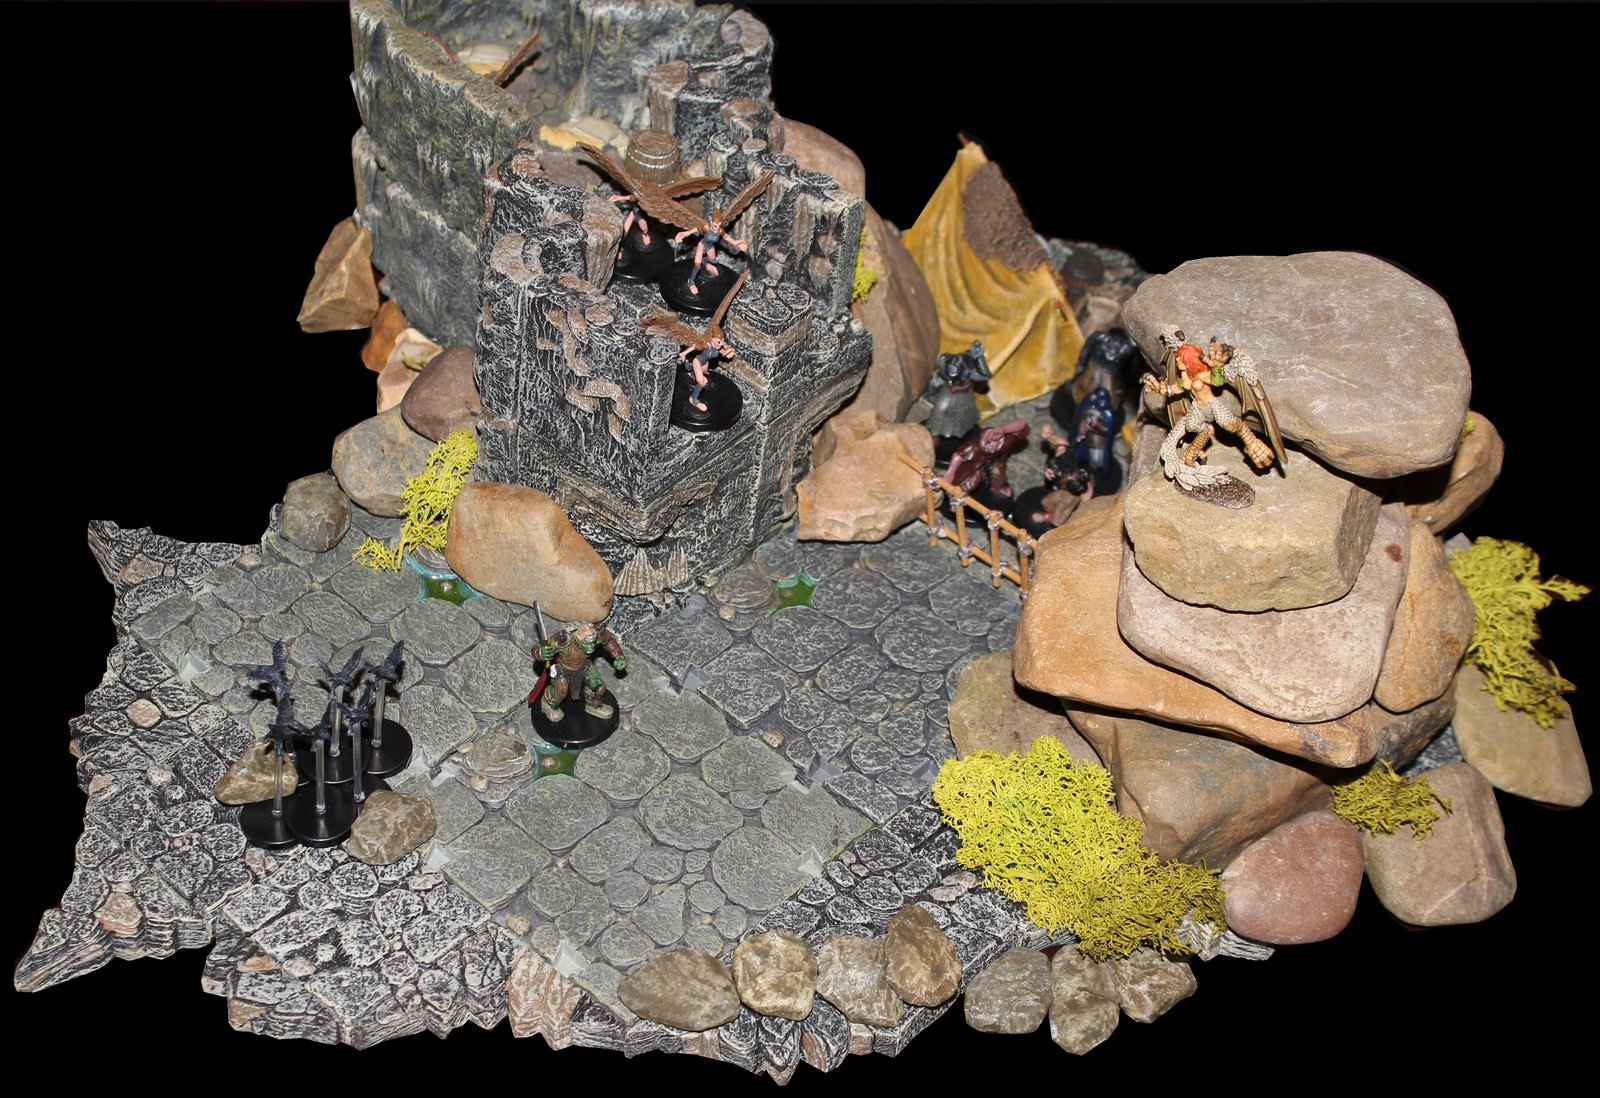
\includegraphics[width=0.39\textwidth]{images/Circeis-lair-for-token-into-Urgir-587600250.jpg}
	\caption{Circeis' lair for token into Urgir}
	\label{fig:Circeis-lair-for-token-into-Urgir-587600250}
\end{figure}

\begin{figure}[h]
	\centering
	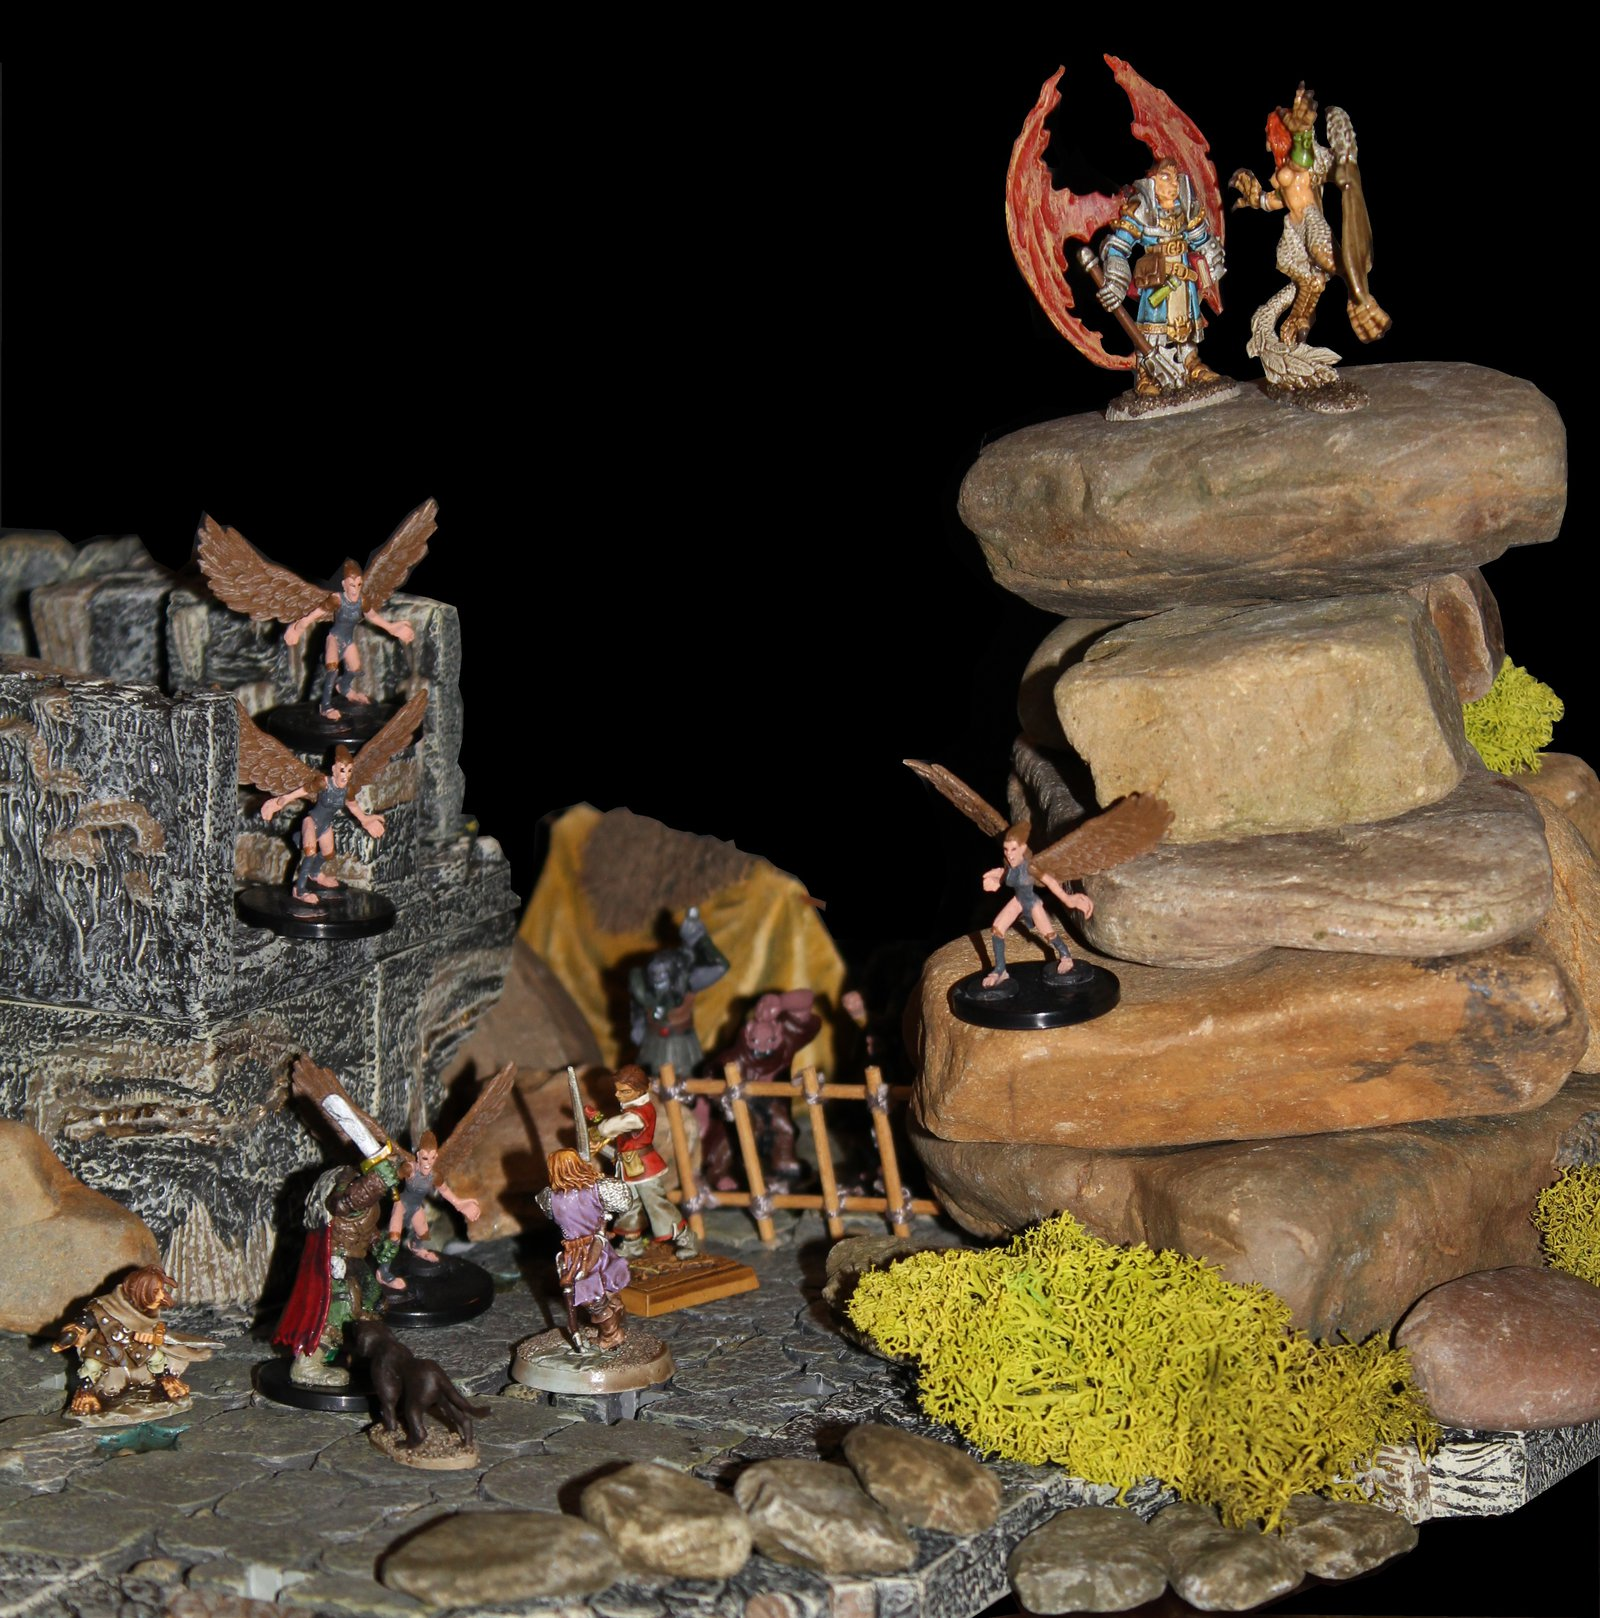
\includegraphics[width=0.39\textwidth]{images/Fighting-the-harpies-in-Circeis-lair-587601733.jpg}
	\caption{Fighting the harpies in Circeis' lair}
	\label{fig:Fighting-the-harpies-in-Circeis-lair-587601733}
\end{figure}

\begin{figure}[h]
	\centering
	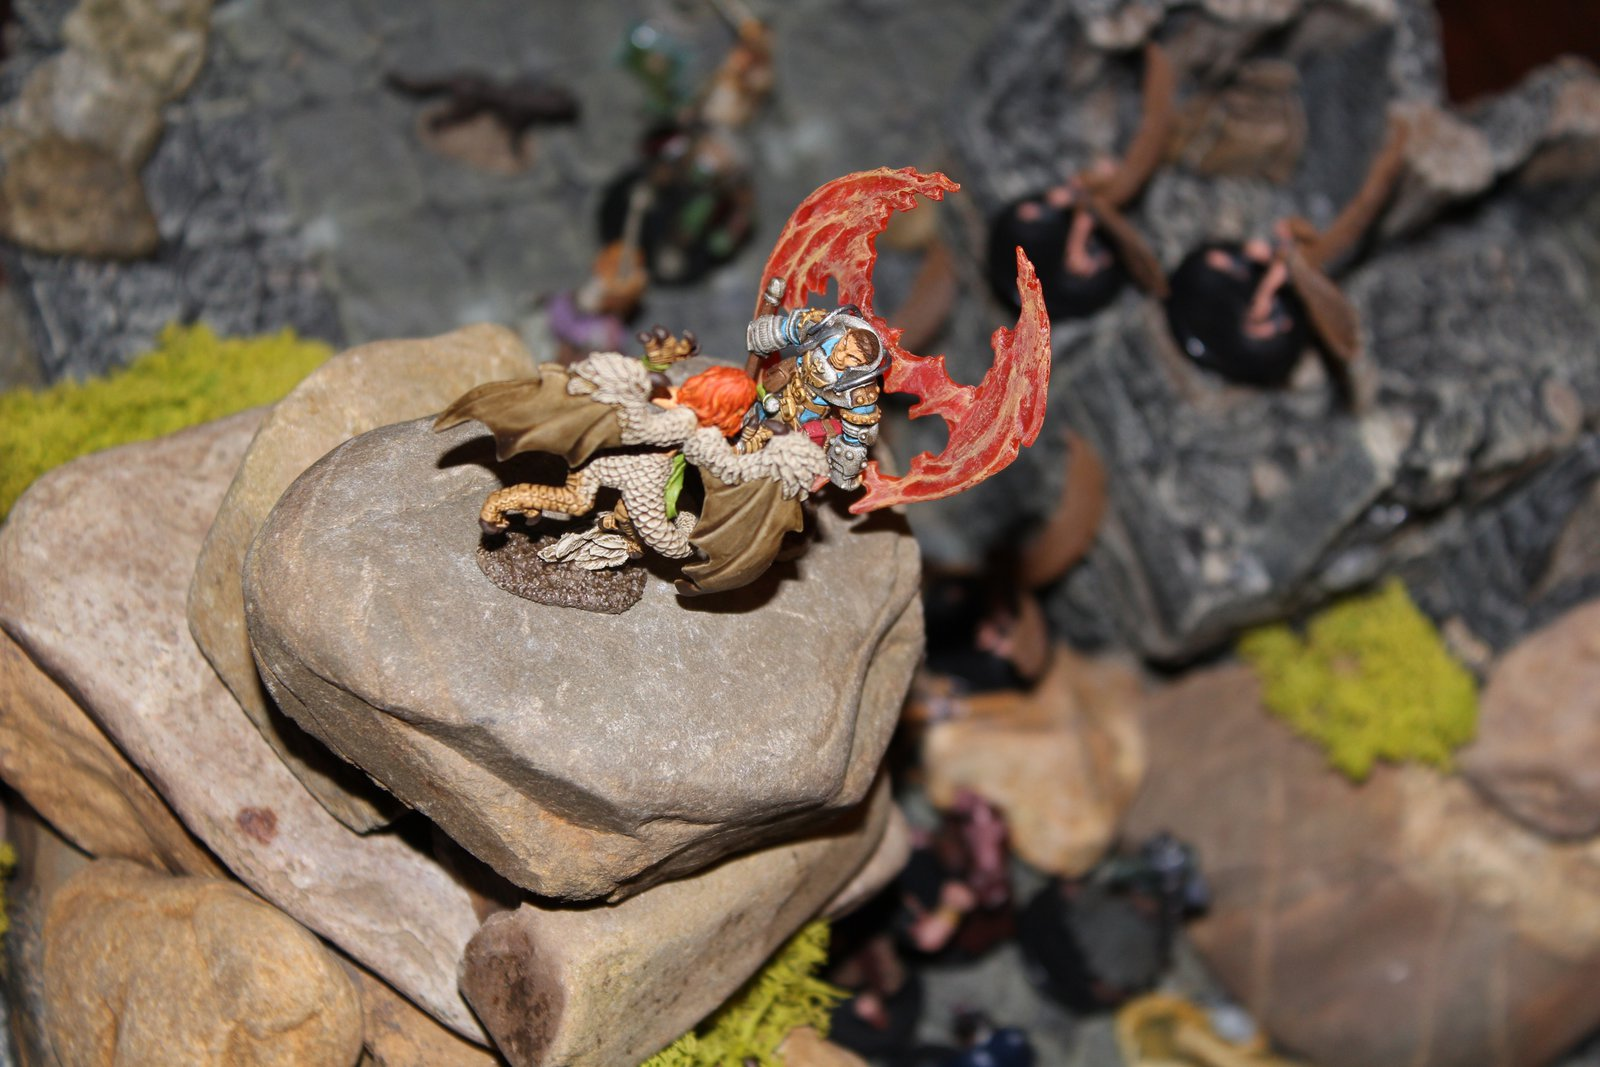
\includegraphics[width=0.39\textwidth]{images/Sjo-confonts-the-harpy-witch-587602339.jpg}
	\caption{Sjo confronts the harpy witch}
	\label{fig:Sjo-confonts-the-harpy-witch-587602339}
\end{figure}

